\begin{figure}[!htb]
    \begin{center}
    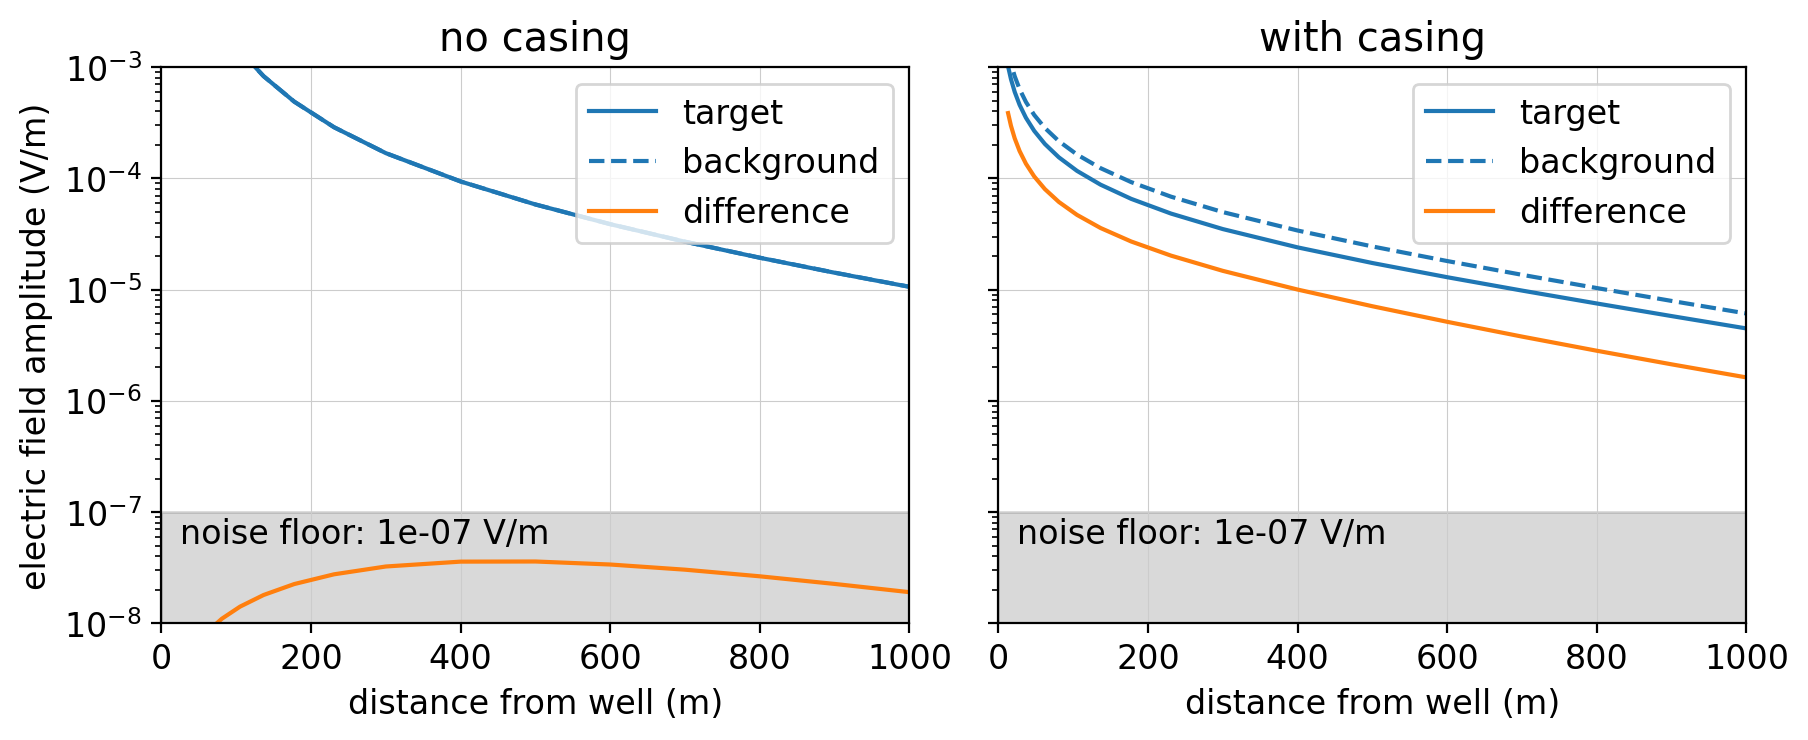
\includegraphics[width=0.8\textwidth]{figures/impact-of-wells-data.png}
    \end{center}
\caption{
    Simulated electric field measurements for the DC resistivity experiment shown in Figure \ref{fig:impact-of-wells}.
    The plots show the data with (solid blue) and without (dashed blue) the target. The orange line is the difference between the two; this is the signal due to the target.
    Without the casing, the response due to the target is below a $10^{-7}$ V/m noise floor, whereas with the casing, the signal is detectable.
}
\label{fig:impact-of-wells-data}
\end{figure}
